\chapter{Implementacija i korisničko sučelje}
		
		
		\section{Korištene tehnologije i alati}
		

			
			 	{U projektu smo koristili različita razvojna okruženja i alate za svaku granu projekta.\\
			 	Za izradu i rad na bazi podataka korišten je alat \textbf{\href{https://www.pgadmin.org/}{pgAdmin}} za rad s \textbf{\href{https://www.postgresql.org/}{PostgreSQL}} tehnologijom,koji je omogućavao lakše praćenje stanje baze i povijest provedenih traženja i postavki u bazi\\
			 	Za \textit{backend} dio projekt korišteno je razvojno okruženje \textbf{\href{https://www.eclipse.org/}{Eclipse}} u kojem je program pisan \textbf{\href{https://www.java.com/en/}{Java}} programskim jezikom sa \textbf{\href{https://spring.io/projects/spring-boot}{Spring boot}} radni okvir sa znatnim programskim kraticama i nadogradnjama, te \textbf{\href{https://maven.apache.org/}{Maven}} podrškom za dohvaćanja programskih ovisnosti u projektu\\
			 	Za \textit{frontend} je korišteno razvojno okruženje \textbf{\href{https://code.visualstudio.com/}{Visual studio code}} u kojem je dodajući ekstenzije bio omogućen bolji rad s tehnologijom \textbf{\href{https://reactjs.org/}{REACT}} koja je znatno ubrzala rad na izgledu i funkcionalnosti stranice prikazane korisniku.
			 	\textbf{\href{https://nodejs.org/en/}{Node.js}} je služio za upravljanjem ostalih programskih ovisnosti u Reactu. \textbf{\href{https://leafletjs.com/}{Leaflet}}-om se dobivaju podaci o karti, a \textbf{\href{http://project-osrm.org/}{OSRM}} za traži put između lokacija.\\
			 	Za međusobno dijeljene koda korištena je tehnologija \textbf{\href{http://www.git-scm.com/}{Git}} te udaljeni repozitorij \textbf{\href{https://about.gitlab.com/}{GitLab}} za svima dostupnu pohranu.\\
			 	Komunikacija pri radu je ostvarena \textbf{\href{https://www.whatsapp.com/}{WhatsApp}} mobilnom aplikacijom za dogovaranje termina i raspodjele obaveza,te \textbf{\href{https://discord.com/}{Discord}} programom za glasovnu komunikaciju pri timskom radu.\\
			 	Za dokumentaciju korišten je alat \textbf{\href{https://tug.org/texlive/}{TexStudio}} u kombinaciji sa TexLive programom koji je generirao PDF dokumente iz .tex datoteka.\\
			 	Za izradu UML dijagrama koristili smo alat \textbf{\href{https://astah.net/}{Astah}} koji smo dobili na korištenje studentskom licencom}.
			
			
			\eject 
		
	\newpage
		\section{Ispitivanje programskog rješenja}
			

			
			{U sljedećem potpoglavlju ispitivanje funkcionalnosti sustava izvedeno je korištenjem ekstenzije za web preglednik "Chrome" pod imenom "Selenium IDE".}
	
			
			\subsection{Ispitivanje komponenti}
			{Pri ispitivanju komponenti ispitani su Obrasci uporabe \textbf{UC1} do \textbf{UC7}. U nastavku su dani kodovi ispitivanja osnovnih funkcionalnih zahtjeva naše aplikacije.}
			
			\newpage
			\begin{packed_item}
				\item {Prikaz koda s kojim je ispitano slanje registracije novog korisnika.}\\
				
				\begin{figure}[h!]
					\centering
					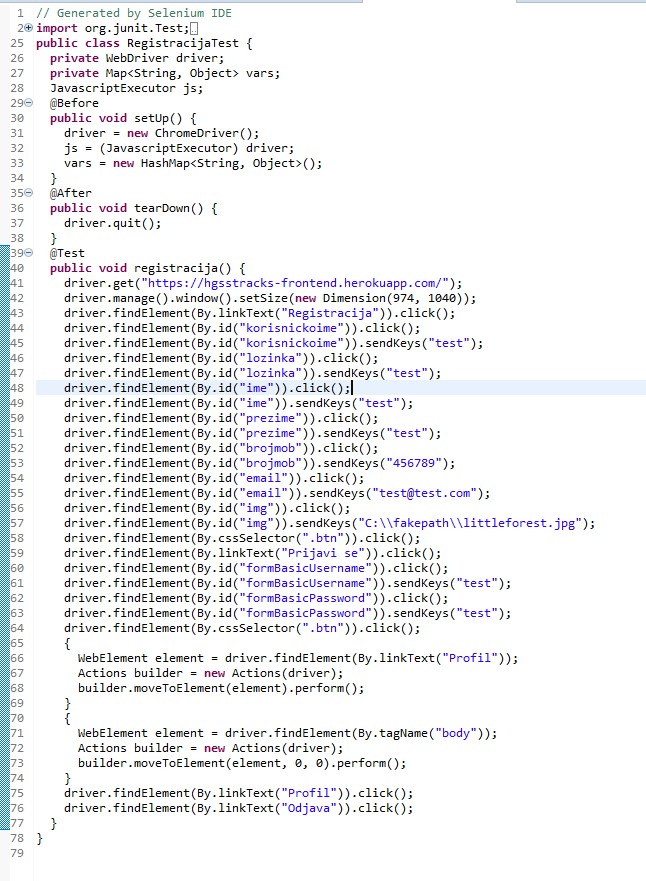
\includegraphics[width=\linewidth]{./slike/TestRegistracije.jpg}
					\caption{Prikaz koda ispitivanja UC1}
				\end{figure}
				\eject
			\end{packed_item}
		
			\newpage
			\begin{packed_item}
				\item {Prikaz koda u kojemu je ispitivan pokušaj prijave u sustav s profilom koji nije bio odobren od strane jednog od admina aplikacije (dodatna mjera sigurnosti).}\\
				
				\begin{figure}[h!]
					\centering
					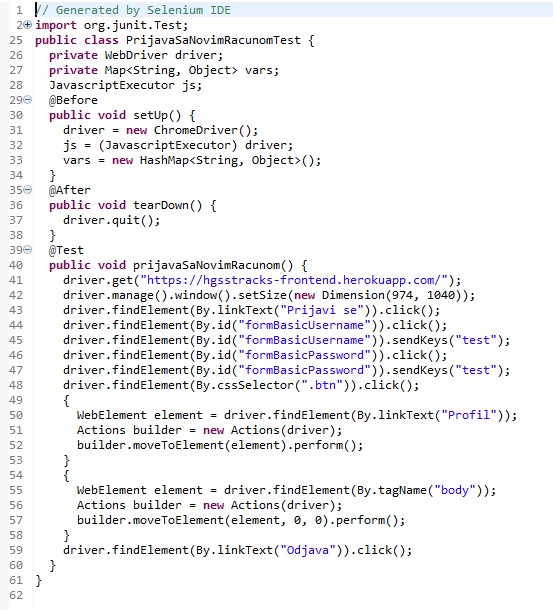
\includegraphics[width=\linewidth]{./slike/PokusajPrijaveSaNepotvdrenimRacunom.jpg}
					\caption{Prikaz koda ispitivanja \textbf{UC4} s kredencijama koje nisu potvrđene od strane admina}
				\end{figure}
				\eject
			\end{packed_item}
		
			\newpage
			\begin{packed_item}
				\item {Prijava u račun jednog od admina te pregled zahtjeva za registraciju i prihvaćanje istog.}\\
				
				\begin{figure}[h!]
					\centering
					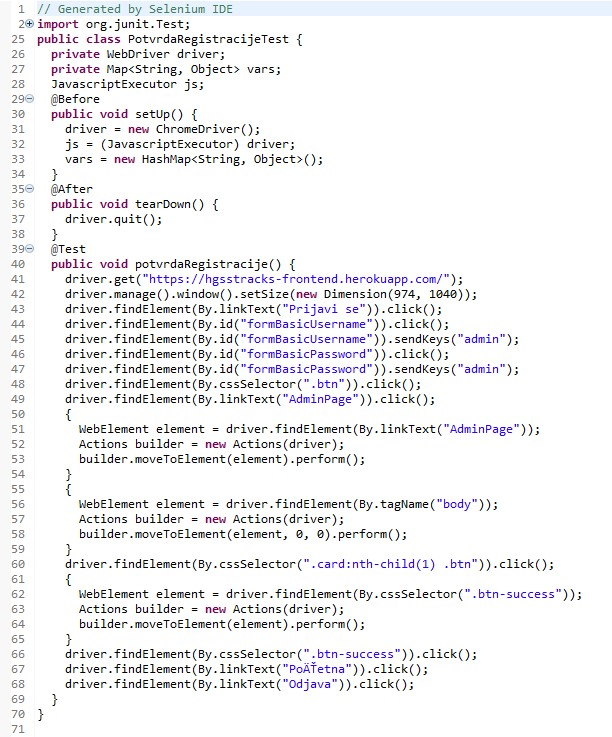
\includegraphics[width=\linewidth]{./slike/ManipulacijaRegistracija.jpg}
					\caption{Prikaz koda ispitivanja \textbf{UC2} i \textbf{UC3}}
				\end{figure}
				\eject
			\end{packed_item}
		
			\newpage
			\begin{packed_item}
				\item {Prijava s novo nastalim profilom (također potvrđenim) te mijenjanje informacija o korisniku, u ovom slučaju izvedena je promjena telefonskog broja spasioca.}\\
				
				\begin{figure}[h!]
					\centering
					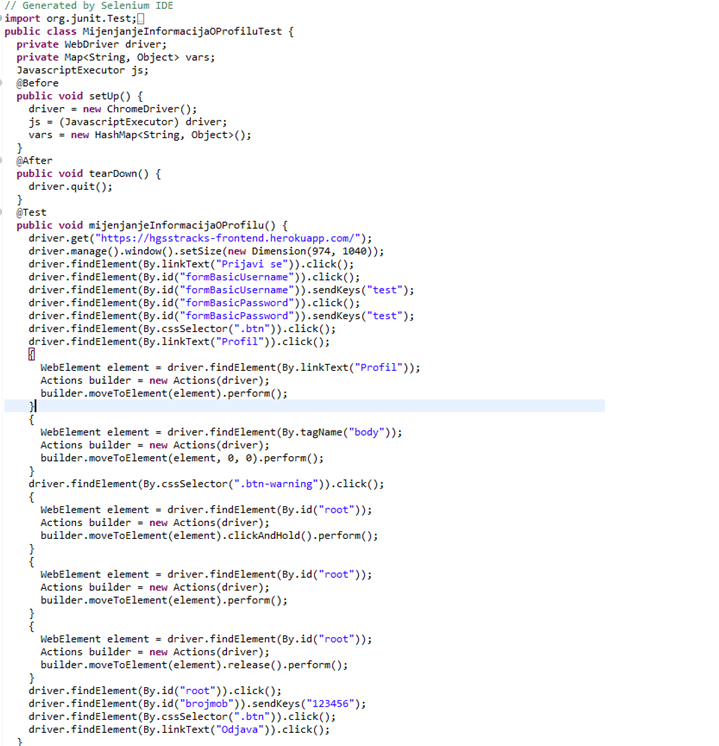
\includegraphics[width=\linewidth]{./slike/Slika2.png}
					\caption{Prikaz koda ispitivanja \textbf{UC4, UC5} i \textbf{UC6}}
				\end{figure}
				\eject
			\end{packed_item}
			\newpage
			
			\begin{packed_item}
				\item {Nakon određenog vremena korištenja profila ispitano je brisanje istog.}\\
				
				\begin{figure}[h!]
					\centering
					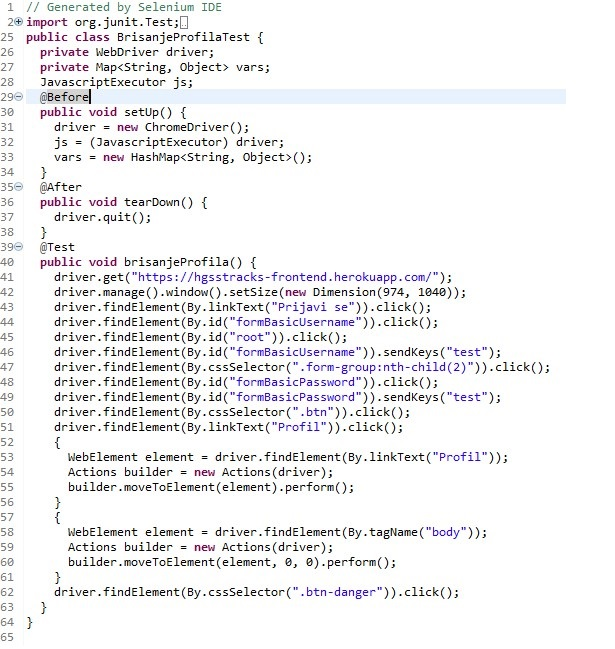
\includegraphics[width=\linewidth]{./slike/BrisanjeProfila.jpg}
					\caption{Prikaz koda ispitivanja \textbf{UC7}}
				\end{figure}
				\eject
			\end{packed_item}
			
			
			
			
			
			
			
			\subsection{Ispitivanje sustava}
			
			 {U sljedećim ispitima funkcionalnosti sustava ispitani su obrasci uporabe \textbf{UC4, UC5,UC24,UC26} i \textbf{UC30}}\\
			 
			 \textbf{Ispitni slučaj 1: Prijava na akciju spašavanja}
			 
			 \textbf{Ulaz:}
			 \begin{itemize}
			 	\item {Prijava u sustav s kredencijama spasioca;}
			 	\item {Pritisak na "Akcije u tijeku" te na jednoj od moguće ponuđenih akcija klik na "Prijavi se na akciju";}
			 	\item {Na "Trenutna Akcija" u \textit{textbox} za ostavljanje komentara ostaviti komentar "SeleniumSelfTest";}
			 	\item {Dojava dispečeru da je osoba pronađena za klikom na gumb "Dojavi".}
			 \end{itemize}
		 	\textbf{Očekivani rezultat:}
		 	\begin{itemize}
		 		\item {Prikazuje se početna stranica;}
		 		\item {Prikazuju se sve aktivne akcije u koje se moguće prijaviti;}
		 		\item {Nakon klika na jednu od akcija očekuje se skočni tekst na samoj stranici koji potvrđuje javljanje na akciju;}
		 		\item {Ostavljanje komentara za dispečera za uvid u akciju na terenu;}
		 		\item {Dojava uspješna da je žrtva nađena.}
		 	\end{itemize}
	 		{\textbf{Rezultat: Svi rezultati su uspješno izvedeni. Aplikacija je prošla test.}}
	 		
			 \begin{figure}[h!]
			 	\centering
			 	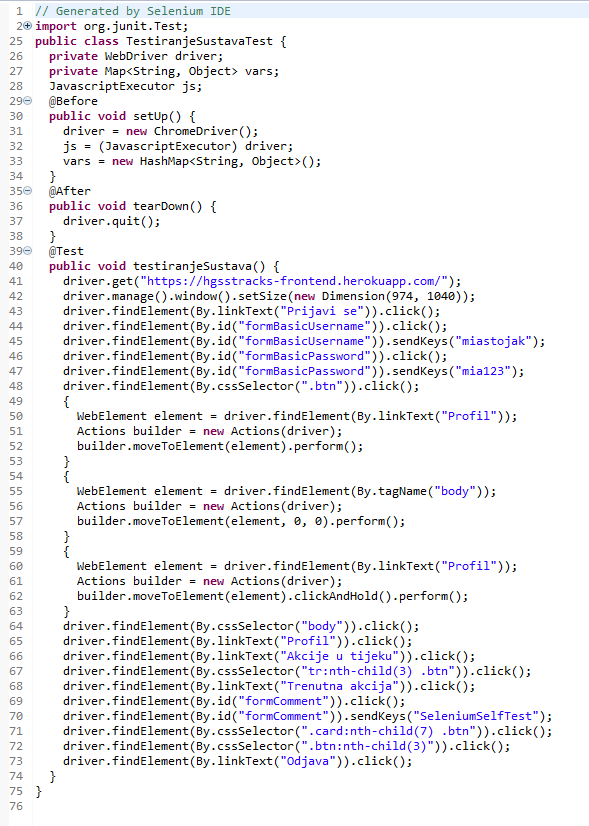
\includegraphics[width=\linewidth]{./slike/IspitivanjeSustava.png}
			 	\caption{Prikaz koda ispitivanja navedenih obrazaca uporabe}
			 \end{figure}
			
			\eject 
			
			\begin{figure}[h!]
				\centering
				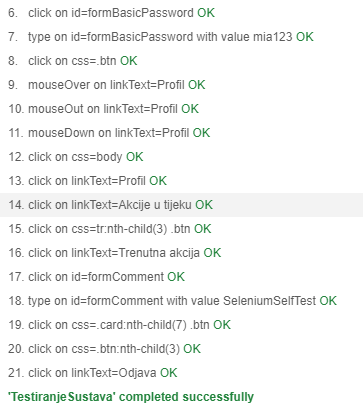
\includegraphics[width=\linewidth]{./slike/TestiranjeRezultat.png}
				\caption{Prikaz Selenium IDE kvalitetu testova}
			\end{figure}
		
			\eject
			
		
		\newpage
		\section{Dijagram razmještaja}
			
			
			 {Dijagram razmještaja na slici ispod prikazuje topologiju komponenti naše aplikacije te programsku potporu iste u radnom okruženju.Na poslužiteljskom računalu se nalazi web poslužitelj aplikacije te baza podataka s informacijama o spasiocima, akcijama, informacijama nestalih osoba, stanicama te ostalih komponenata bitnih za kvalitetan rad aplikacije. Korisnici aplikacije koriste web preglednik kako bi pristupili aplikaciji. Sustav naše aplikacije je baziran na arhitekturi "klijent-poslužitelj", a komunikacija između računala korisnika i poslužitelja odvija se preko HTTP veze.}
			 
			 \begin{figure}[h!]
			 	\centering
			 	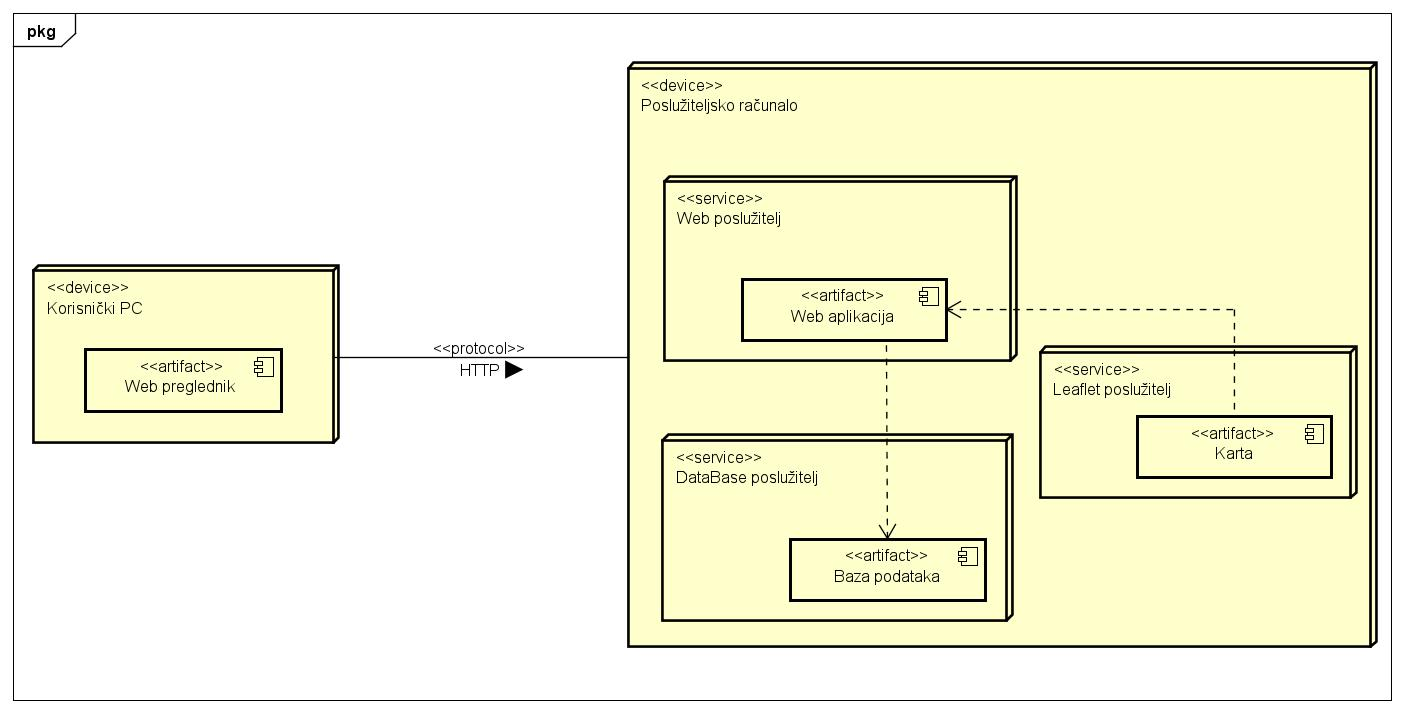
\includegraphics[width=\linewidth]{./slike/Dijagram_razmjestaja.jpg}
			 	\caption{Dijagram razmještaja komponenti}
			 \end{figure}
			
			\eject 
		
		\section{Upute za puštanje u pogon}
		
			\textbf{Instalacija poslužitelja baze podataka}\\
		
			 {Potrebno je preuzeti SQL Shell(Postgress SQL) bazu podataka te pgAdmin radi lakše manipulacije s podatcima tj. bolje preglednosti. Nakon preuzimanja paketa potrebno je provesti standardnu instalaciju s postavljanjem korisnika.}\\
			 
			 \textbf{Konfiguracija poslužitelja baze podataka}\\
			 
			 {Nakon instalacije, uključite pgAdmin server te izvršite prvu konekciju na bazu (s postavljanjem \textit{master} zaporke za pristup).}\\
			 
			 \textbf{Punjenje baze s informacijama}\\
			 
			 {Po prvom paljenju servera baze podataka potrebno je pomoću nekog od uređivača tekstova(notepad,notepad++ itd.) otvoriti datoteku po imenu "Baza.sql" te označiti cijeli tekst i kopirati ga. Kada ste kopirali konfiguraciju baze iz datoteke. Na web poslužitelju pgAdmin potrebno je u padajućem izborniku za "PostgreSQL 13" kliknuti desni klik miša te ići na "New database" te na skočnom prozoru  upisati ime baze, u ovom slučaju "Baza korisnika" te stisnuti "Create". Po izradi baze desni klik na bazu te "Query tool" i na novom prozoru koji će se pojaviti na desnoj strani ekrana zalijepiti tekst iz datoteke "Baza.sql" i pritisnuti gumb "Run".}\\
			 
			 \textbf{Instalacija poslužitelja \textit{backend} koda}\\
			 
			 {Potrebno je preuzeti Eclipse za službene stranice proizvoda. Nakon što se program preuzme potrebno je izvršiti standardnu instalaciju. Također je potrebno u "System variables" postaviti putanju za JAVA HOME.}\\
			 
			 \textbf{Postavljanje putanje za JAVU}\\
			 
			 {Potrebno je otići na "This PC" - desni klik na "This PC" - "Properties" - "Advanced system settings" - "Enviromental variables" - Dvoklik na "Path" - "New". Kada se napravi nova linija potrebno je u nju kopirati tekst "\%JAVA\_HOME\%\textbackslash bin". Nakon toga potrebno je u "Enviromental variables" na donjem dijelu prozoru gdje je "System variables" kliknuti "New" te u "Variable name" upisati "JAVA\_HOME", a u "Variable value" putanju gdje je instaliran JAVA paket na vašem računalu.}\\
			 
			 \textbf{Dodavanje ekstenzija na Eclipse}\\
			 
			 {Nakon instalacije programa Eclipse, te namještanja putanje za JAVA\_HOME potrebno je upaliti program te ići na karticu "Help" - "Eclipse Marketplace" te u find \textit{textboxu} upisati "spring" i instalirati \textit{dashboard} za "Spring Tools 3"(ili trenutnu verziju programa). Nakon instalacije \textit{dashboard}-a potrebno je otići na \textit{\href{https://maven.apache.org/install.html}{https://maven.apache.org/install.html}} te preuzeti paket i instalirati ga na računalo.}\\
			 
			 \textbf{\textit{Importanje backend} dijela aplikacije u Eclipse}\\
			 
			 {Po instalaciji svih potrebnih programa i ekstenzija za \textit{backend} dio aplikacije, otvorite program Eclipse te na kartici "File" - "Import" - "Maven" - "Existing Maven Projects" - "Next" - "Browse" i u skočnom prozoru pronaći datoteku u kojoj je spremljen kod te "Finish". Projektni dio koda je ubačen u Eclipse i moguće je manipulirati s kodom.}\\
			 
			 \textbf{Instalacija \textit{frontend} poslužitelja}\\
			 
			 {Kako bismo mogli vidjeti te preuređivati \textit{frontend} kod potrebno je instalirati program \textit{\textbf{Visual Studio Code}} sa \href{https://code.visualstudio.com/Download}{https://code.visualstudio.com/Download}.}\\
			 
			 \textbf{Instalacija REACT biblioteke u Visual Studio Code program}\\
			 
			 {U svakoj datoteci vezanoj za \textit{frontend} kod potrebno je na početku upisati komande: 
			 import React from 'react';
		 	 import ReactDOM from 'react-dom';
	 	 	 nakon što smo upisali ove dvije komade moguće je koristiti REACT biblioteku u daljnjem kodu.}\\
			
			\textbf{\textit{Importanje frontend} dijela koda u program}\\
			
			{Po instalaciji programa "Visual Studio Code" upalite program te "File" - "Open" te označiti mapu u kojoj se nalaze sve datoteke \textit{frontend} dijela projekta. Po uspješnom otvaranju datoteka moguće je manipulirati kodom.}\\
			
			\textbf{\textit{Deploy backend} dijela projekta na Heroku}\\
			
			{U datoteku "pom.xml" potrebno je dodati maven plugin za \textbf{Heroku} čiji je dependency moguće naći na \href{https://elements.heroku.com/buildpacks/heroku/heroku-maven-plugin}{ovom linku}. Nakon dodavanja "dependency-ja" upalite git bash te se pozicionirati u mapu u kojoj se nalazi projekt. U "Git-bash" je potrebno upisati naredbu heroku git:remote -a hgsstracks-backend. Informacije o bazi podataka za aplikaciju moguće je naredbom heroku pg:info. Iz informacija koje smo dobili o bazi podataka potrebno je iščitati <Add-on>. Kada smo iščitali <Add-on> napunićemo bazu podataka informacijama koje imamo u mapi "Izvršni kod" upišemo naredbu heroku pg:psql <Add-on> --app <name\_of\_app> < my\_sql\_file.sql;, u našem slučaju ta naredba glasi heroku pg:psql postgresql-curly-47290 --app hgsstracks-backend < Baza.sql. U datoteci application.properties je potrebno postaviti informacije o bazi tj. ime baze podataka te zaporku za istu koju smo postavili u prethodnim koracima. Nakon punjenja baze pozovemo naredbu mvn clean heroku:deploy te je s time \textit{backend} dio projekta pušten u pogon.}\\
			
			\textbf{\textit{Deploy frontend} dijela projekta na Heroku}\\
			
			{U vršnu mapu projekta potrebno je dodati datoteku "package.json" s naredbama "heroku-prebuild": "cd \"Izvorni kod"/frontend/hgsstracks\" i start": "start": "cd \"Izvorni kod"/frontend/hgsstracks/\" \&\& npm start" te naposljetku "build": "cd \"Izvorni kod"/frontend/hgsstracks\" \&\& react-scripts build". Nakon izvedbe naredbi u "package.json" unutar \textit{frontend} mape potrebno je promijeniti skripte u "start": "npm install -g serve \&\& serve -s build". Upalimo "Git-bash" te se pozicioniramo u njemu u mapu u kojoj se nalazi naš \textit{frontend} dio projekta te upišemo naredbu heroku git:remote -a hgsstracks-frontend. Pozovemo naredbu git push heroku <branch>:main, u našem slučaju ta naredba je git push heroku develop:main. \textit{Frontend} dio projekta je pušten u pogon.}\\
			
			
			
			
			\eject 